\documentclass{standalone}
\usepackage{tikz}
\usetikzlibrary{patterns, positioning}


\begin{document}
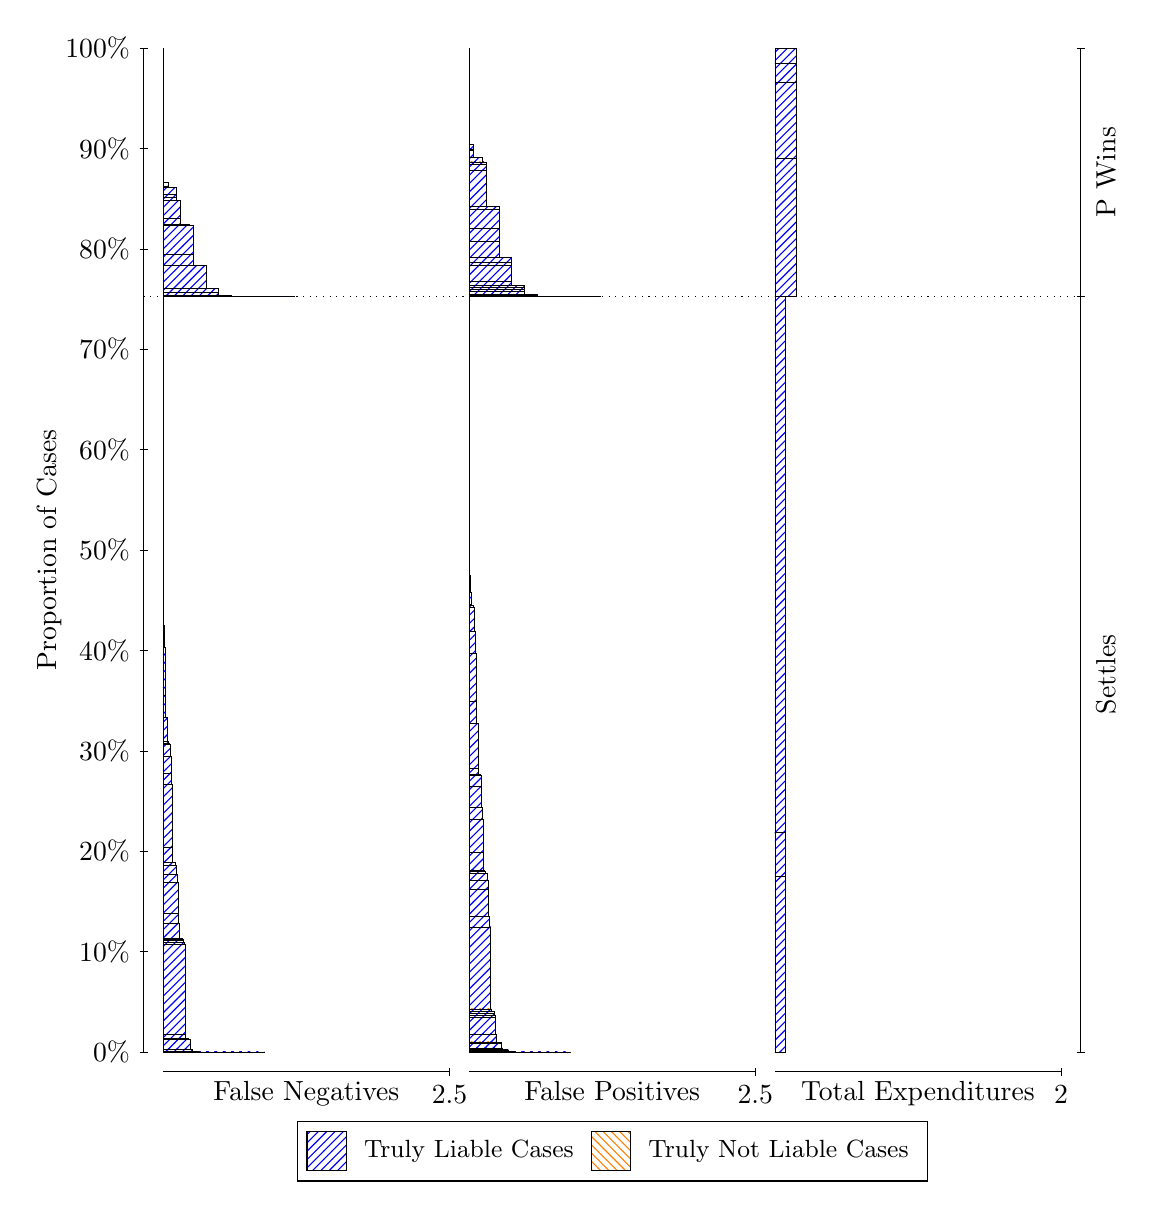
\begin{tikzpicture}
\draw[black, very thin] (1.5,1.75) -- (1.5,14.5);
\node[rotate=90, text=black, anchor=center] at (0.3, 8.125) {Proportion of Cases};
\draw[black, very thin] (1.45,1.75) -- (1.55,1.75);
\node[text=black, anchor=east] at (1.45, 1.75) {0\%};
\draw[black, very thin] (1.45,3.025) -- (1.55,3.025);
\node[text=black, anchor=east] at (1.45, 3.025) {10\%};
\draw[black, very thin] (1.45,4.3) -- (1.55,4.3);
\node[text=black, anchor=east] at (1.45, 4.3) {20\%};
\draw[black, very thin] (1.45,5.575) -- (1.55,5.575);
\node[text=black, anchor=east] at (1.45, 5.575) {30\%};
\draw[black, very thin] (1.45,6.85) -- (1.55,6.85);
\node[text=black, anchor=east] at (1.45, 6.85) {40\%};
\draw[black, very thin] (1.45,8.125) -- (1.55,8.125);
\node[text=black, anchor=east] at (1.45, 8.125) {50\%};
\draw[black, very thin] (1.45,9.4) -- (1.55,9.4);
\node[text=black, anchor=east] at (1.45, 9.4) {60\%};
\draw[black, very thin] (1.45,10.675) -- (1.55,10.675);
\node[text=black, anchor=east] at (1.45, 10.675) {70\%};
\draw[black, very thin] (1.45,11.95) -- (1.55,11.95);
\node[text=black, anchor=east] at (1.45, 11.95) {80\%};
\draw[black, very thin] (1.45,13.225) -- (1.55,13.225);
\node[text=black, anchor=east] at (1.45, 13.225) {90\%};
\draw[black, very thin] (1.45,14.5) -- (1.55,14.5);
\node[text=black, anchor=east] at (1.45, 14.5) {100\%};

\draw[black, very thin] (13.4,1.75) -- (13.4,14.5);
\draw[black, very thin] (13.35,1.75) -- (13.45,1.75);
\node[anchor=west] at (13.35, 1.75) {};
\draw[black, very thin] (13.35,11.343) -- (13.45,11.343);
\node[anchor=west] at (13.35, 11.343) {};
\draw[black, very thin] (13.35,14.5) -- (13.45,14.5);
\node[anchor=west] at (13.35, 14.5) {};

\draw[black, very thin, pattern color=blue, pattern=north east lines] (1.75,1.75) rectangle (3.0398,1.75);
\draw[black, very thin, pattern color=blue, pattern=north east lines] (1.75,1.75) rectangle (2.9672,1.75);
\draw[black, very thin, pattern color=blue, pattern=north east lines] (1.75,1.75) rectangle (2.8945,1.75);
\draw[black, very thin, pattern color=blue, pattern=north east lines] (1.75,1.75) rectangle (2.8784,1.75);
\draw[black, very thin, pattern color=blue, pattern=north east lines] (1.75,1.75) rectangle (2.8218,1.75);
\draw[black, very thin, pattern color=blue, pattern=north east lines] (1.75,1.75) rectangle (2.8057,1.75);
\draw[black, very thin, pattern color=blue, pattern=north east lines] (1.75,1.75) rectangle (2.7492,1.75);
\draw[black, very thin, pattern color=blue, pattern=north east lines] (1.75,1.75) rectangle (2.733,1.75);
\draw[black, very thin, pattern color=blue, pattern=north east lines] (1.75,1.75) rectangle (2.7169,1.75);
\draw[black, very thin, pattern color=blue, pattern=north east lines] (1.75,1.75) rectangle (2.6765,1.75);
\draw[black, very thin, pattern color=blue, pattern=north east lines] (1.75,1.75) rectangle (2.6604,1.75);
\draw[black, very thin, pattern color=blue, pattern=north east lines] (1.75,1.75) rectangle (2.6442,1.75);
\draw[black, very thin, pattern color=blue, pattern=north east lines] (1.75,1.75) rectangle (2.6038,1.75);
\draw[black, very thin, pattern color=blue, pattern=north east lines] (1.75,1.75) rectangle (2.5877,1.75);
\draw[black, very thin, pattern color=blue, pattern=north east lines] (1.75,1.75) rectangle (2.5715,1.75);
\draw[black, very thin, pattern color=blue, pattern=north east lines] (1.75,1.75) rectangle (2.5554,1.75);
\draw[black, very thin, pattern color=blue, pattern=north east lines] (1.75,1.75) rectangle (2.5312,1.75);
\draw[black, very thin, pattern color=blue, pattern=north east lines] (1.75,1.75) rectangle (2.515,1.75);
\draw[black, very thin, pattern color=blue, pattern=north east lines] (1.75,1.75) rectangle (2.4989,1.75);
\draw[black, very thin, pattern color=blue, pattern=north east lines] (1.75,1.75) rectangle (2.4827,1.75);
\draw[black, very thin, pattern color=blue, pattern=north east lines] (1.75,1.75) rectangle (2.4585,1.75);
\draw[black, very thin, pattern color=blue, pattern=north east lines] (1.75,1.75) rectangle (2.4424,1.75);
\draw[black, very thin, pattern color=blue, pattern=north east lines] (1.75,1.75) rectangle (2.4262,1.75);
\draw[black, very thin, pattern color=blue, pattern=north east lines] (1.75,1.75) rectangle (2.4101,1.75);
\draw[black, very thin, pattern color=blue, pattern=north east lines] (1.75,1.75) rectangle (2.3939,1.75);
\draw[black, very thin, pattern color=blue, pattern=north east lines] (1.75,1.75) rectangle (2.3858,1.75);
\draw[black, very thin, pattern color=blue, pattern=north east lines] (1.75,1.75) rectangle (2.3697,1.75);
\draw[black, very thin, pattern color=blue, pattern=north east lines] (1.75,1.75) rectangle (2.3535,1.75);
\draw[black, very thin, pattern color=blue, pattern=north east lines] (1.75,1.75) rectangle (2.3374,1.75);
\draw[black, very thin, pattern color=blue, pattern=north east lines] (1.75,1.75) rectangle (2.3212,1.75);
\draw[black, very thin, pattern color=blue, pattern=north east lines] (1.75,1.75) rectangle (2.3132,1.75);
\draw[black, very thin, pattern color=blue, pattern=north east lines] (1.75,1.75) rectangle (2.297,1.75);
\draw[black, very thin, pattern color=blue, pattern=north east lines] (1.75,1.75) rectangle (2.2809,1.7505);
\draw[black, very thin, pattern color=blue, pattern=north east lines] (1.75,1.7505) rectangle (2.2647,1.7507);
\draw[black, very thin, pattern color=blue, pattern=north east lines] (1.75,1.7507) rectangle (2.2486,1.7507);
\draw[black, very thin, pattern color=blue, pattern=north east lines] (1.75,1.7507) rectangle (2.2324,1.7508);
\draw[black, very thin, pattern color=blue, pattern=north east lines] (1.75,1.7508) rectangle (2.2244,1.7508);
\draw[black, very thin, pattern color=blue, pattern=north east lines] (1.75,1.7508) rectangle (2.2082,1.7508);
\draw[black, very thin, pattern color=blue, pattern=north east lines] (1.75,1.7508) rectangle (2.1921,1.7531);
\draw[black, very thin, pattern color=blue, pattern=north east lines] (1.75,1.7531) rectangle (2.1759,1.7538);
\draw[black, very thin, pattern color=blue, pattern=north east lines] (1.75,1.7538) rectangle (2.1678,1.7548);
\draw[black, very thin, pattern color=blue, pattern=north east lines] (1.75,1.7548) rectangle (2.1598,1.7553);
\draw[black, very thin, pattern color=blue, pattern=north east lines] (1.75,1.7553) rectangle (2.1517,1.7556);
\draw[black, very thin, pattern color=blue, pattern=north east lines] (1.75,1.7556) rectangle (2.1355,1.7557);
\draw[black, very thin, pattern color=blue, pattern=north east lines] (1.75,1.7557) rectangle (2.1194,1.7791);
\draw[black, very thin, pattern color=blue, pattern=north east lines] (1.75,1.7791) rectangle (2.1032,1.7885);
\draw[black, very thin, pattern color=blue, pattern=north east lines] (1.75,1.7885) rectangle (2.0952,1.9106);
\draw[black, very thin, pattern color=blue, pattern=north east lines] (1.75,1.9106) rectangle (2.0871,1.9172);
\draw[black, very thin, pattern color=blue, pattern=north east lines] (1.75,1.9172) rectangle (2.0709,1.9228);
\draw[black, very thin, pattern color=blue, pattern=north east lines] (1.75,1.9228) rectangle (2.0629,1.9249);
\draw[black, very thin, pattern color=blue, pattern=north east lines] (1.75,1.9249) rectangle (2.0467,1.925);
\draw[black, very thin, pattern color=blue, pattern=north east lines] (1.75,1.925) rectangle (2.0306,1.9733);
\draw[black, very thin, pattern color=blue, pattern=north east lines] (1.75,1.9733) rectangle (2.0225,3.1148);
\draw[black, very thin, pattern color=blue, pattern=north east lines] (1.75,3.1148) rectangle (2.0144,3.1384);
\draw[black, very thin, pattern color=blue, pattern=north east lines] (1.75,3.1384) rectangle (2.0064,3.1657);
\draw[black, very thin, pattern color=blue, pattern=north east lines] (1.75,3.1657) rectangle (1.9983,3.1863);
\draw[black, very thin, pattern color=blue, pattern=north east lines] (1.75,3.1863) rectangle (1.9902,3.1915);
\draw[black, very thin, pattern color=blue, pattern=north east lines] (1.75,3.1915) rectangle (1.9741,3.1946);
\draw[black, very thin, pattern color=blue, pattern=north east lines] (1.75,3.1946) rectangle (1.9579,3.3871);
\draw[black, very thin, pattern color=blue, pattern=north east lines] (1.75,3.3871) rectangle (1.9418,3.5099);
\draw[black, very thin, pattern color=blue, pattern=north east lines] (1.75,3.5099) rectangle (1.9337,3.901);
\draw[black, very thin, pattern color=blue, pattern=north east lines] (1.75,3.901) rectangle (1.9256,4.0081);
\draw[black, very thin, pattern color=blue, pattern=north east lines] (1.75,4.0081) rectangle (1.9095,4.1261);
\draw[black, very thin, pattern color=blue, pattern=north east lines] (1.75,4.1261) rectangle (1.9014,4.158);
\draw[black, very thin, pattern color=blue, pattern=north east lines] (1.75,4.158) rectangle (1.8852,4.1599);
\draw[black, very thin, pattern color=blue, pattern=north east lines] (1.75,4.1599) rectangle (1.8691,4.3524);
\draw[black, very thin, pattern color=blue, pattern=north east lines] (1.75,4.3524) rectangle (1.861,5.1448);
\draw[black, very thin, pattern color=blue, pattern=north east lines] (1.75,5.1448) rectangle (1.8529,5.2885);
\draw[black, very thin, pattern color=blue, pattern=north east lines] (1.75,5.2885) rectangle (1.8449,5.5024);
\draw[black, very thin, pattern color=blue, pattern=north east lines] (1.75,5.5024) rectangle (1.8368,5.6518);
\draw[black, very thin, pattern color=blue, pattern=north east lines] (1.75,5.6518) rectangle (1.8287,5.6756);
\draw[black, very thin, pattern color=blue, pattern=north east lines] (1.75,5.6756) rectangle (1.8126,5.6948);
\draw[black, very thin, pattern color=blue, pattern=north east lines] (1.75,5.6948) rectangle (1.7964,6.0003);
\draw[black, very thin, pattern color=blue, pattern=north east lines] (1.75,6.0003) rectangle (1.7803,6.2806);
\draw[black, very thin, pattern color=blue, pattern=north east lines] (1.75,6.2806) rectangle (1.7722,6.8868);
\draw[black, very thin, pattern color=blue, pattern=north east lines] (1.75,6.8868) rectangle (1.7641,7.1704);
\draw[black, very thin, pattern color=orange, pattern=north west lines] (1.75,7.1704) rectangle (1.75,7.1704);
\draw[black, very thin, pattern color=blue, pattern=north east lines] (1.75,7.1704) rectangle (1.75,11.343);
\draw[black, very thin, pattern color=blue, pattern=north east lines] (1.75,11.343) rectangle (3.4213,11.343);
\draw[black, very thin, pattern color=blue, pattern=north east lines] (1.75,11.343) rectangle (3.2599,11.343);
\draw[black, very thin, pattern color=blue, pattern=north east lines] (1.75,11.343) rectangle (3.2599,11.343);
\draw[black, very thin, pattern color=blue, pattern=north east lines] (1.75,11.343) rectangle (3.0984,11.343);
\draw[black, very thin, pattern color=blue, pattern=north east lines] (1.75,11.343) rectangle (3.0984,11.343);
\draw[black, very thin, pattern color=blue, pattern=north east lines] (1.75,11.343) rectangle (2.9369,11.343);
\draw[black, very thin, pattern color=blue, pattern=north east lines] (1.75,11.343) rectangle (2.8804,11.343);
\draw[black, very thin, pattern color=blue, pattern=north east lines] (1.75,11.343) rectangle (2.7754,11.344);
\draw[black, very thin, pattern color=blue, pattern=north east lines] (1.75,11.344) rectangle (2.7754,11.345);
\draw[black, very thin, pattern color=blue, pattern=north east lines] (1.75,11.345) rectangle (2.7189,11.345);
\draw[black, very thin, pattern color=blue, pattern=north east lines] (1.75,11.345) rectangle (2.7189,11.345);
\draw[black, very thin, pattern color=blue, pattern=north east lines] (1.75,11.345) rectangle (2.6139,11.361);
\draw[black, very thin, pattern color=blue, pattern=north east lines] (1.75,11.361) rectangle (2.5574,11.361);
\draw[black, very thin, pattern color=blue, pattern=north east lines] (1.75,11.361) rectangle (2.4524,11.392);
\draw[black, very thin, pattern color=blue, pattern=north east lines] (1.75,11.392) rectangle (2.4524,11.449);
\draw[black, very thin, pattern color=blue, pattern=north east lines] (1.75,11.449) rectangle (2.3959,11.449);
\draw[black, very thin, pattern color=blue, pattern=north east lines] (1.75,11.449) rectangle (2.3959,11.449);
\draw[black, very thin, pattern color=blue, pattern=north east lines] (1.75,11.449) rectangle (2.291,11.743);
\draw[black, very thin, pattern color=blue, pattern=north east lines] (1.75,11.743) rectangle (2.2344,11.744);
\draw[black, very thin, pattern color=blue, pattern=north east lines] (1.75,11.744) rectangle (2.2344,11.744);
\draw[black, very thin, pattern color=blue, pattern=north east lines] (1.75,11.744) rectangle (2.2344,11.744);
\draw[black, very thin, pattern color=blue, pattern=north east lines] (1.75,11.744) rectangle (2.1295,11.881);
\draw[black, very thin, pattern color=blue, pattern=north east lines] (1.75,11.881) rectangle (2.1295,12.243);
\draw[black, very thin, pattern color=blue, pattern=north east lines] (1.75,12.243) rectangle (2.073,12.244);
\draw[black, very thin, pattern color=blue, pattern=north east lines] (1.75,12.244) rectangle (2.073,12.259);
\draw[black, very thin, pattern color=blue, pattern=north east lines] (1.75,12.259) rectangle (1.968,12.332);
\draw[black, very thin, pattern color=blue, pattern=north east lines] (1.75,12.332) rectangle (1.968,12.568);
\draw[black, very thin, pattern color=blue, pattern=north east lines] (1.75,12.568) rectangle (1.9115,12.607);
\draw[black, very thin, pattern color=blue, pattern=north east lines] (1.75,12.607) rectangle (1.9115,12.641);
\draw[black, very thin, pattern color=blue, pattern=north east lines] (1.75,12.641) rectangle (1.9115,12.735);
\draw[black, very thin, pattern color=blue, pattern=north east lines] (1.75,12.735) rectangle (1.8065,12.735);
\draw[black, very thin, pattern color=blue, pattern=north east lines] (1.75,12.735) rectangle (1.8065,12.741);
\draw[black, very thin, pattern color=blue, pattern=north east lines] (1.75,12.741) rectangle (1.8065,12.789);
\draw[black, very thin, pattern color=blue, pattern=north east lines] (1.75,12.789) rectangle (1.8065,12.789);
\draw[black, very thin, pattern color=orange, pattern=north west lines] (1.75,12.789) rectangle (1.75,12.789);
\draw[black, very thin, pattern color=blue, pattern=north east lines] (1.75,12.789) rectangle (1.75,14.5);
\draw[black, very thin, pattern color=orange, pattern=north west lines] (5.6333,1.75) rectangle (6.9232,1.75);
\draw[black, very thin, pattern color=blue, pattern=north east lines] (5.6333,1.75) rectangle (6.9232,1.75);
\draw[black, very thin, pattern color=orange, pattern=north west lines] (5.6333,1.75) rectangle (6.8505,1.75);
\draw[black, very thin, pattern color=blue, pattern=north east lines] (5.6333,1.75) rectangle (6.8505,1.75);
\draw[black, very thin, pattern color=orange, pattern=north west lines] (5.6333,1.75) rectangle (6.7778,1.75);
\draw[black, very thin, pattern color=blue, pattern=north east lines] (5.6333,1.75) rectangle (6.7778,1.75);
\draw[black, very thin, pattern color=blue, pattern=north east lines] (5.6333,1.75) rectangle (6.7617,1.75);
\draw[black, very thin, pattern color=blue, pattern=north east lines] (5.6333,1.75) rectangle (6.689,1.75);
\draw[black, very thin, pattern color=orange, pattern=north west lines] (5.6333,1.75) rectangle (6.6325,1.75);
\draw[black, very thin, pattern color=blue, pattern=north east lines] (5.6333,1.75) rectangle (6.6325,1.75);
\draw[black, very thin, pattern color=blue, pattern=north east lines] (5.6333,1.75) rectangle (6.6164,1.75);
\draw[black, very thin, pattern color=blue, pattern=north east lines] (5.6333,1.75) rectangle (6.6002,1.75);
\draw[black, very thin, pattern color=orange, pattern=north west lines] (5.6333,1.75) rectangle (6.5598,1.75);
\draw[black, very thin, pattern color=blue, pattern=north east lines] (5.6333,1.75) rectangle (6.5598,1.75);
\draw[black, very thin, pattern color=blue, pattern=north east lines] (5.6333,1.75) rectangle (6.5275,1.75);
\draw[black, very thin, pattern color=orange, pattern=north west lines] (5.6333,1.75) rectangle (6.4872,1.75);
\draw[black, very thin, pattern color=blue, pattern=north east lines] (5.6333,1.75) rectangle (6.4872,1.75);
\draw[black, very thin, pattern color=blue, pattern=north east lines] (5.6333,1.75) rectangle (6.471,1.75);
\draw[black, very thin, pattern color=blue, pattern=north east lines] (5.6333,1.75) rectangle (6.4549,1.75);
\draw[black, very thin, pattern color=blue, pattern=north east lines] (5.6333,1.75) rectangle (6.4387,1.75);
\draw[black, very thin, pattern color=orange, pattern=north west lines] (5.6333,1.75) rectangle (6.4145,1.75);
\draw[black, very thin, pattern color=blue, pattern=north east lines] (5.6333,1.75) rectangle (6.4145,1.75);
\draw[black, very thin, pattern color=blue, pattern=north east lines] (5.6333,1.75) rectangle (6.3984,1.75);
\draw[black, very thin, pattern color=blue, pattern=north east lines] (5.6333,1.75) rectangle (6.3661,1.75);
\draw[black, very thin, pattern color=orange, pattern=north west lines] (5.6333,1.75) rectangle (6.3418,1.75);
\draw[black, very thin, pattern color=blue, pattern=north east lines] (5.6333,1.75) rectangle (6.3418,1.75);
\draw[black, very thin, pattern color=blue, pattern=north east lines] (5.6333,1.75) rectangle (6.3257,1.75);
\draw[black, very thin, pattern color=blue, pattern=north east lines] (5.6333,1.75) rectangle (6.3095,1.75);
\draw[black, very thin, pattern color=blue, pattern=north east lines] (5.6333,1.75) rectangle (6.2934,1.7505);
\draw[black, very thin, pattern color=blue, pattern=north east lines] (5.6333,1.7505) rectangle (6.2772,1.7505);
\draw[black, very thin, pattern color=orange, pattern=north west lines] (5.6333,1.7505) rectangle (6.2692,1.7505);
\draw[black, very thin, pattern color=blue, pattern=north east lines] (5.6333,1.7505) rectangle (6.2692,1.7505);
\draw[black, very thin, pattern color=blue, pattern=north east lines] (5.6333,1.7505) rectangle (6.253,1.7505);
\draw[black, very thin, pattern color=blue, pattern=north east lines] (5.6333,1.7505) rectangle (6.2369,1.7506);
\draw[black, very thin, pattern color=blue, pattern=north east lines] (5.6333,1.7506) rectangle (6.2046,1.753);
\draw[black, very thin, pattern color=orange, pattern=north west lines] (5.6333,1.753) rectangle (6.1965,1.753);
\draw[black, very thin, pattern color=blue, pattern=north east lines] (5.6333,1.753) rectangle (6.1965,1.7531);
\draw[black, very thin, pattern color=blue, pattern=north east lines] (5.6333,1.7531) rectangle (6.1804,1.7532);
\draw[black, very thin, pattern color=blue, pattern=north east lines] (5.6333,1.7532) rectangle (6.1642,1.7533);
\draw[black, very thin, pattern color=blue, pattern=north east lines] (5.6333,1.7533) rectangle (6.1481,1.7533);
\draw[black, very thin, pattern color=blue, pattern=north east lines] (5.6333,1.7533) rectangle (6.1319,1.7772);
\draw[black, very thin, pattern color=orange, pattern=north west lines] (5.6333,1.7772) rectangle (6.1238,1.7772);
\draw[black, very thin, pattern color=blue, pattern=north east lines] (5.6333,1.7772) rectangle (6.1238,1.7785);
\draw[black, very thin, pattern color=blue, pattern=north east lines] (5.6333,1.7785) rectangle (6.1158,1.779);
\draw[black, very thin, pattern color=blue, pattern=north east lines] (5.6333,1.779) rectangle (6.1077,1.7796);
\draw[black, very thin, pattern color=blue, pattern=north east lines] (5.6333,1.7796) rectangle (6.0915,1.7797);
\draw[black, very thin, pattern color=blue, pattern=north east lines] (5.6333,1.7797) rectangle (6.0754,1.7817);
\draw[black, very thin, pattern color=orange, pattern=north west lines] (5.6333,1.7817) rectangle (6.0512,1.7817);
\draw[black, very thin, pattern color=blue, pattern=north east lines] (5.6333,1.7817) rectangle (6.0512,1.8014);
\draw[black, very thin, pattern color=blue, pattern=north east lines] (5.6333,1.8014) rectangle (6.0431,1.8598);
\draw[black, very thin, pattern color=blue, pattern=north east lines] (5.6333,1.8598) rectangle (6.035,1.8673);
\draw[black, very thin, pattern color=blue, pattern=north east lines] (5.6333,1.8673) rectangle (6.0189,1.8726);
\draw[black, very thin, pattern color=blue, pattern=north east lines] (5.6333,1.8726) rectangle (6.0027,1.8756);
\draw[black, very thin, pattern color=blue, pattern=north east lines] (5.6333,1.8756) rectangle (5.9866,1.8787);
\draw[black, very thin, pattern color=orange, pattern=north west lines] (5.6333,1.8787) rectangle (5.9785,1.8787);
\draw[black, very thin, pattern color=blue, pattern=north east lines] (5.6333,1.8787) rectangle (5.9785,1.9796);
\draw[black, very thin, pattern color=blue, pattern=north east lines] (5.6333,1.9796) rectangle (5.9704,2.1908);
\draw[black, very thin, pattern color=blue, pattern=north east lines] (5.6333,2.1908) rectangle (5.9624,2.2179);
\draw[black, very thin, pattern color=blue, pattern=north east lines] (5.6333,2.2179) rectangle (5.9543,2.2441);
\draw[black, very thin, pattern color=blue, pattern=north east lines] (5.6333,2.2441) rectangle (5.9462,2.2649);
\draw[black, very thin, pattern color=blue, pattern=north east lines] (5.6333,2.2649) rectangle (5.9301,2.2667);
\draw[black, very thin, pattern color=blue, pattern=north east lines] (5.6333,2.2667) rectangle (5.9139,2.2982);
\draw[black, very thin, pattern color=orange, pattern=north west lines] (5.6333,2.2982) rectangle (5.9058,2.2982);
\draw[black, very thin, pattern color=blue, pattern=north east lines] (5.6333,2.2982) rectangle (5.9058,3.3388);
\draw[black, very thin, pattern color=blue, pattern=north east lines] (5.6333,3.3388) rectangle (5.8897,3.4797);
\draw[black, very thin, pattern color=blue, pattern=north east lines] (5.6333,3.4797) rectangle (5.8816,3.8205);
\draw[black, very thin, pattern color=blue, pattern=north east lines] (5.6333,3.8205) rectangle (5.8735,3.9288);
\draw[black, very thin, pattern color=blue, pattern=north east lines] (5.6333,3.9288) rectangle (5.8574,4.0225);
\draw[black, very thin, pattern color=blue, pattern=north east lines] (5.6333,4.0225) rectangle (5.8412,4.0417);
\draw[black, very thin, pattern color=blue, pattern=north east lines] (5.6333,4.0417) rectangle (5.8251,4.0623);
\draw[black, very thin, pattern color=blue, pattern=north east lines] (5.6333,4.0623) rectangle (5.817,4.2834);
\draw[black, very thin, pattern color=blue, pattern=north east lines] (5.6333,4.2834) rectangle (5.8089,4.7066);
\draw[black, very thin, pattern color=blue, pattern=north east lines] (5.6333,4.7066) rectangle (5.8009,4.852);
\draw[black, very thin, pattern color=blue, pattern=north east lines] (5.6333,4.852) rectangle (5.7928,5.1195);
\draw[black, very thin, pattern color=blue, pattern=north east lines] (5.6333,5.1195) rectangle (5.7847,5.2672);
\draw[black, very thin, pattern color=blue, pattern=north east lines] (5.6333,5.2672) rectangle (5.7686,5.2719);
\draw[black, very thin, pattern color=blue, pattern=north east lines] (5.6333,5.2719) rectangle (5.7524,5.3516);
\draw[black, very thin, pattern color=blue, pattern=north east lines] (5.6333,5.3516) rectangle (5.7444,5.9228);
\draw[black, very thin, pattern color=blue, pattern=north east lines] (5.6333,5.9228) rectangle (5.7282,6.2065);
\draw[black, very thin, pattern color=blue, pattern=north east lines] (5.6333,6.2065) rectangle (5.7201,6.8127);
\draw[black, very thin, pattern color=blue, pattern=north east lines] (5.6333,6.8127) rectangle (5.7121,7.093);
\draw[black, very thin, pattern color=blue, pattern=north east lines] (5.6333,7.093) rectangle (5.6959,7.3984);
\draw[black, very thin, pattern color=blue, pattern=north east lines] (5.6333,7.3984) rectangle (5.6798,7.4176);
\draw[black, very thin, pattern color=blue, pattern=north east lines] (5.6333,7.4176) rectangle (5.6636,7.4414);
\draw[black, very thin, pattern color=blue, pattern=north east lines] (5.6333,7.4414) rectangle (5.6555,7.5909);
\draw[black, very thin, pattern color=blue, pattern=north east lines] (5.6333,7.5909) rectangle (5.6475,7.8047);
\draw[black, very thin, pattern color=blue, pattern=north east lines] (5.6333,7.8047) rectangle (5.6394,7.9485);
\draw[black, very thin, pattern color=blue, pattern=north east lines] (5.6333,7.9485) rectangle (5.6333,11.343);
\draw[black, very thin, pattern color=orange, pattern=north west lines] (5.6333,11.343) rectangle (7.3047,11.343);
\draw[black, very thin, pattern color=blue, pattern=north east lines] (5.6333,11.343) rectangle (7.3047,11.343);
\draw[black, very thin, pattern color=orange, pattern=north west lines] (5.6333,11.343) rectangle (7.1432,11.343);
\draw[black, very thin, pattern color=blue, pattern=north east lines] (5.6333,11.343) rectangle (7.1432,11.343);
\draw[black, very thin, pattern color=orange, pattern=north west lines] (5.6333,11.343) rectangle (6.9817,11.343);
\draw[black, very thin, pattern color=blue, pattern=north east lines] (5.6333,11.343) rectangle (6.9817,11.343);
\draw[black, very thin, pattern color=blue, pattern=north east lines] (5.6333,11.343) rectangle (6.9817,11.343);
\draw[black, very thin, pattern color=blue, pattern=north east lines] (5.6333,11.343) rectangle (6.9817,11.343);
\draw[black, very thin, pattern color=orange, pattern=north west lines] (5.6333,11.343) rectangle (6.8202,11.343);
\draw[black, very thin, pattern color=blue, pattern=north east lines] (5.6333,11.343) rectangle (6.8202,11.343);
\draw[black, very thin, pattern color=blue, pattern=north east lines] (5.6333,11.343) rectangle (6.8202,11.343);
\draw[black, very thin, pattern color=orange, pattern=north west lines] (5.6333,11.343) rectangle (6.6587,11.343);
\draw[black, very thin, pattern color=blue, pattern=north east lines] (5.6333,11.343) rectangle (6.6587,11.344);
\draw[black, very thin, pattern color=blue, pattern=north east lines] (5.6333,11.344) rectangle (6.6587,11.346);
\draw[black, very thin, pattern color=orange, pattern=north west lines] (5.6333,11.346) rectangle (6.6022,11.346);
\draw[black, very thin, pattern color=blue, pattern=north east lines] (5.6333,11.346) rectangle (6.6022,11.346);
\draw[black, very thin, pattern color=blue, pattern=north east lines] (5.6333,11.346) rectangle (6.4973,11.353);
\draw[black, very thin, pattern color=orange, pattern=north west lines] (5.6333,11.353) rectangle (6.4973,11.353);
\draw[black, very thin, pattern color=blue, pattern=north east lines] (5.6333,11.353) rectangle (6.4973,11.358);
\draw[black, very thin, pattern color=blue, pattern=north east lines] (5.6333,11.358) rectangle (6.4973,11.368);
\draw[black, very thin, pattern color=orange, pattern=north west lines] (5.6333,11.368) rectangle (6.4407,11.368);
\draw[black, very thin, pattern color=blue, pattern=north east lines] (5.6333,11.368) rectangle (6.4407,11.368);
\draw[black, very thin, pattern color=blue, pattern=north east lines] (5.6333,11.368) rectangle (6.3358,11.407);
\draw[black, very thin, pattern color=blue, pattern=north east lines] (5.6333,11.407) rectangle (6.3358,11.438);
\draw[black, very thin, pattern color=orange, pattern=north west lines] (5.6333,11.438) rectangle (6.3358,11.438);
\draw[black, very thin, pattern color=blue, pattern=north east lines] (5.6333,11.438) rectangle (6.3358,11.461);
\draw[black, very thin, pattern color=blue, pattern=north east lines] (5.6333,11.461) rectangle (6.3358,11.485);
\draw[black, very thin, pattern color=blue, pattern=north east lines] (5.6333,11.485) rectangle (6.2793,11.485);
\draw[black, very thin, pattern color=orange, pattern=north west lines] (5.6333,11.485) rectangle (6.2793,11.485);
\draw[black, very thin, pattern color=blue, pattern=north east lines] (5.6333,11.485) rectangle (6.2793,11.485);
\draw[black, very thin, pattern color=blue, pattern=north east lines] (5.6333,11.485) rectangle (6.1743,11.537);
\draw[black, very thin, pattern color=orange, pattern=north west lines] (5.6333,11.537) rectangle (6.1743,11.537);
\draw[black, very thin, pattern color=blue, pattern=north east lines] (5.6333,11.537) rectangle (6.1743,11.738);
\draw[black, very thin, pattern color=blue, pattern=north east lines] (5.6333,11.738) rectangle (6.1743,11.779);
\draw[black, very thin, pattern color=blue, pattern=north east lines] (5.6333,11.779) rectangle (6.1743,11.844);
\draw[black, very thin, pattern color=blue, pattern=north east lines] (5.6333,11.844) rectangle (6.1178,11.844);
\draw[black, very thin, pattern color=orange, pattern=north west lines] (5.6333,11.844) rectangle (6.1178,11.844);
\draw[black, very thin, pattern color=blue, pattern=north east lines] (5.6333,11.844) rectangle (6.1178,11.844);
\draw[black, very thin, pattern color=blue, pattern=north east lines] (5.6333,11.844) rectangle (6.0128,12.043);
\draw[black, very thin, pattern color=blue, pattern=north east lines] (5.6333,12.043) rectangle (6.0128,12.208);
\draw[black, very thin, pattern color=blue, pattern=north east lines] (5.6333,12.208) rectangle (6.0128,12.451);
\draw[black, very thin, pattern color=blue, pattern=north east lines] (5.6333,12.451) rectangle (6.0128,12.491);
\draw[black, very thin, pattern color=blue, pattern=north east lines] (5.6333,12.491) rectangle (5.9563,12.491);
\draw[black, very thin, pattern color=orange, pattern=north west lines] (5.6333,12.491) rectangle (5.9563,12.491);
\draw[black, very thin, pattern color=blue, pattern=north east lines] (5.6333,12.491) rectangle (5.9563,12.491);
\draw[black, very thin, pattern color=blue, pattern=north east lines] (5.6333,12.491) rectangle (5.8513,12.953);
\draw[black, very thin, pattern color=blue, pattern=north east lines] (5.6333,12.953) rectangle (5.8513,13.03);
\draw[black, very thin, pattern color=blue, pattern=north east lines] (5.6333,13.03) rectangle (5.8513,13.054);
\draw[black, very thin, pattern color=blue, pattern=north east lines] (5.6333,13.054) rectangle (5.7948,13.054);
\draw[black, very thin, pattern color=orange, pattern=north west lines] (5.6333,13.054) rectangle (5.7948,13.054);
\draw[black, very thin, pattern color=blue, pattern=north east lines] (5.6333,13.054) rectangle (5.7948,13.108);
\draw[black, very thin, pattern color=blue, pattern=north east lines] (5.6333,13.108) rectangle (5.7948,13.108);
\draw[black, very thin, pattern color=blue, pattern=north east lines] (5.6333,13.108) rectangle (5.6899,13.202);
\draw[black, very thin, pattern color=blue, pattern=north east lines] (5.6333,13.202) rectangle (5.6899,13.219);
\draw[black, very thin, pattern color=blue, pattern=north east lines] (5.6333,13.219) rectangle (5.6899,13.272);
\draw[black, very thin, pattern color=blue, pattern=north east lines] (5.6333,13.272) rectangle (5.6899,13.275);
\draw[black, very thin, pattern color=orange, pattern=north west lines] (5.6333,13.275) rectangle (5.6333,13.275);
\draw[black, very thin, pattern color=blue, pattern=north east lines] (5.6333,13.275) rectangle (5.6333,14.5);
\draw[black, very thin, pattern color=orange, pattern=north west lines] (9.5167,1.75) rectangle (9.6529,1.75);
\draw[black, very thin, pattern color=blue, pattern=north east lines] (9.5167,1.75) rectangle (9.6529,3.978);
\draw[black, very thin, pattern color=orange, pattern=north west lines] (9.5167,3.978) rectangle (9.6529,3.978);
\draw[black, very thin, pattern color=blue, pattern=north east lines] (9.5167,3.978) rectangle (9.6529,4.5361);
\draw[black, very thin, pattern color=orange, pattern=north west lines] (9.5167,4.5361) rectangle (9.6529,4.5361);
\draw[black, very thin, pattern color=blue, pattern=north east lines] (9.5167,4.5361) rectangle (9.6529,11.343);
\draw[black, very thin, pattern color=orange, pattern=north west lines] (9.5167,11.343) rectangle (9.7892,11.343);
\draw[black, very thin, pattern color=blue, pattern=north east lines] (9.5167,11.343) rectangle (9.7892,13.099);
\draw[black, very thin, pattern color=orange, pattern=north west lines] (9.5167,13.099) rectangle (9.7892,13.099);
\draw[black, very thin, pattern color=blue, pattern=north east lines] (9.5167,13.099) rectangle (9.7892,14.065);
\draw[black, very thin, pattern color=orange, pattern=north west lines] (9.5167,14.065) rectangle (9.7892,14.065);
\draw[black, very thin, pattern color=blue, pattern=north east lines] (9.5167,14.065) rectangle (9.7892,14.3);
\draw[black, very thin, pattern color=orange, pattern=north west lines] (9.5167,14.3) rectangle (9.7892,14.3);
\draw[black, very thin, pattern color=blue, pattern=north east lines] (9.5167,14.3) rectangle (9.7892,14.5);
\draw[black, dotted] (1.5,11.343) -- (13.4,11.343);
\draw[black, very thin] (1.75,1.5) -- (5.3833,1.5);
\node[text=black, anchor=north] at (3.5667, 1.5) {False Negatives};
\draw[black, very thin] (5.3833,1.45) -- (5.3833,1.55);
\node[text=black, anchor=north] at (5.3833, 1.45) {2.5};

\draw[black, very thin] (5.6333,1.5) -- (9.2667,1.5);
\node[text=black, anchor=north] at (7.45, 1.5) {False Positives};
\draw[black, very thin] (9.2667,1.45) -- (9.2667,1.55);
\node[text=black, anchor=north] at (9.2667, 1.45) {2.5};

\draw[black, very thin] (9.5167,1.5) -- (13.15,1.5);
\node[text=black, anchor=north] at (11.333, 1.5) {Total Expenditures};
\draw[black, very thin] (13.15,1.45) -- (13.15,1.55);
\node[text=black, anchor=north] at (13.15, 1.45) {2};

\node[text=black, centered, rotate=90] at (13.72, 6.5466) {Settles};
\node[text=black, centered, rotate=90] at (13.72, 12.922) {P Wins};

\draw (7.449999999999999,1.5) node[draw=none] (baseCoordinate) {};
\begin{scope}[align=center]
        \matrix[scale=0.5, draw=black, below=0.5cm of baseCoordinate, nodes={draw}, column sep=0.1cm]{
            \node[rectangle, draw, minimum width=0.5cm, minimum height=0.5cm, pattern color=blue, pattern=north east lines] {}; &
            \node[draw=none, font=\small, text=black] (B) {Truly Liable Cases}; &
            \node[rectangle, draw, minimum width=0.5cm, minimum height=0.5cm, pattern color=orange, pattern=north west lines] {}; &
            \node[draw=none, font=\small, text=black] (B) {Truly Not Liable Cases}; \\
            };
\end{scope}

\end{tikzpicture}
\end{document}